% !TeX TS-program = xelatex

\documentclass{resume}
\ResumeName{Ziyu Chen}

\usepackage{graphicx}
\usepackage{tikz}
\usepackage{fontawesome5}

% Personal homepage (custom domain on GitHub Pages)
\newcommand{\MyHomepage}{ziyuchen.me}

\linespread{1.0}

\begin{document}

\ResumeContacts{
  M.Sc. candidate,%
  +86 185-8289-4157,%
  \ResumeUrl{mailto:chenziyu089@163.com}{chenziyu089@163.com},%
  \faHome~\ResumeUrl{https://\MyHomepage}{\MyHomepage}%
}

% Photo pinned to the top-right corner, outside the text flow
\begin{tikzpicture}[remember picture, overlay]
  \node[anchor=north east, xshift=-0.65cm, yshift=-0.35cm]
    at (current page.north east)
    {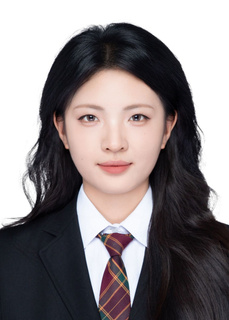
\includegraphics[width=2.0cm]{photo.jpg}};
\end{tikzpicture}%

\ResumeTitle

\section{Education}

\ResumeItem
[University of Electronic Science and Technology of China]
{University of Electronic Science and Technology of China}
[M.Sc., Economics \& Management]
[2024—2027]

\begin{itemize}
  \item \textbf{Honors:} First-Class \& Second-Class School Scholarships; ranked \textbf{1st} in the national entrance examination (cross-disciplinary)
  \item \textbf{Coursework:} Management Information Systems, Data \& Algorithm Governance; research focus: data governance
  \item \textbf{Publication:} \textit{FedLing: Linguistic-Structure-Aware Federated Learning for Fair Multilingual LLM Adaptation}, \textbf{EMNLP 2026 Findings}
\end{itemize}

\ResumeItem
[Shanghai Normal University]
{Shanghai Normal University}
[\textnormal{B.A. in} Tourism Management]
[2020.09—2024.07]

\begin{itemize}
  \item \textbf{Honors:} University scholarship (1$\times$), school scholarships (2$\times$); First Prize (individual), Shanghai ``Starlight Plan'' Skills Competition; coursework in Management, Marketing and Economics
\end{itemize}

\section{Experience}

\ResumeItem
[Trip.com Group|Product Operations Intern]
{Trip.com Group (Shanghai HQ)}
[\textnormal{Overseas Business Unit | Product Operations Intern}]
[2024.05—2024.09]

\begin{itemize}

\item \textbf{Google-channel product development.} Translated Google platform requirements into feature scopes, data definitions and acceptance criteria with internal product and engineering teams; shipped 2 features on schedule (multi-day pass, Google Discover content integration), lifting attraction content exposure by \textbf{11\%}.

\item \textbf{Funnel analysis \& product iteration.} Tracked search interest, exposure and conversion via Google Trends, Search Console and business data; identified \textbf{3+} growth opportunities monthly, pushed 2 proposals (real-time availability, bundled ticketing) into research, raising target-page conversion by \textbf{$\sim$6\%}.

\item \textbf{Cross-platform data governance.} Mapped and validated \textbf{20+} key fields (name, price, inventory, refund policy) between Google and internal systems; led first-time onboarding of \textbf{55} high-potential attractions (Tokyo Disneyland, Colosseum). Delivered \textbf{30+} listing tasks monthly at \textbf{183\%} of target with zero major data errors; bounce rate \textbf{-6\%}, channel conversion \textbf{+3\%}.

\item \textbf{Issue triage \& closure.} Categorized high-frequency issues (inventory sync, API failures, missing confirmations) under a 2-hour response / 8-hour solution standard; closed \textbf{60+} issues within \textbf{12 hours}, turning recurring problems into data rules and product improvements.

\end{itemize}

\ResumeItem
[Chengdu China International Travel Service|Marketing Intern]
{Chengdu China International Travel Service}
[\textnormal{Marketing Intern}]
[2023.09—2024.02]

\begin{itemize}

\item \textbf{Community growth \& campaigns.} Designed WeChat campaigns (Moments sharing, red-packet rain) for new-product launch, reviewing performance through a reach--join--consult funnel: \textbf{15,000+} reach, \textbf{200+} inquiries, \textbf{235} day-one signups (\textbf{117\%} of target), growing the community by nearly \textbf{14k} members in 3 months.

\item \textbf{Needs analysis \& conversion.} Segmented travelers by schedule, budget, destination and party composition; independently closed \textbf{16} customized travel orders end-to-end.

\end{itemize}

\section{Leadership}

\begin{itemize}
  \item \textbf{Graduate Student Union Officer} (awarded ``Outstanding Officer''), UESTC --- organized 4 university-level events for 2,000+ graduate students
  \item \textbf{Student Union Presidium Member} \& \textbf{Class Youth League Secretary} (4 years), Shanghai Normal University --- led 7 university-level cultural events for 5,000+ attendees; organized 13 themed class events
\end{itemize}

\section{Skills}

\begin{itemize}
  \item \textbf{Data \& Analytics:} SQL, Python (Pandas), Excel, Google Analytics, Google Trends, Google Search Console
  \item \textbf{Product Design:} Axure, Figma, Modao, Lanhu, XMind, Photoshop; requirements analysis, flow design, prototyping and PRDs
  \item \textbf{Product Methods:} competitive analysis, user personas, A/B testing, data-driven iteration
  \item \textbf{Collaboration:} JIRA, Confluence, TAPD, Lark, Agile / Scrum
  \item \textbf{AI Tooling:} Claude Code, Codex and other AI agents for requirement analysis, rapid prototyping and data processing
  \item \textbf{Languages \& Certificates:} Mandarin (native), English (CET-6); National Tour Guide License, Computer Level 1
\end{itemize}

\section{Summary}

\begin{itemize}
  \item \textbf{Data-driven:} locate problems and validate results with data; drove exposure +11\% and conversion +6\% via data monitoring
  \item \textbf{Communication:} coordinated with 60+ stakeholders, mobilizing internal and external resources to land requirements
  \item \textbf{Fast learner:} ranked 1st in the cross-disciplinary entrance exam; ramps up fast on complex product logic
  \item \textbf{Business sense:} management background with user insight and internet monetization knowledge\end{itemize}

\end{document}
